% 2장 제도와 선행연구. 출처: docs/prior_work.md · 0010 · 0022 · 0028

\section{제도와 선행연구}

\subsection{토지거래허가제}

토허제의 법적 근거는 「부동산 거래신고 등에 관한 법률」이다. 지정된 구역 안에서
\textbf{일정 면적을 넘는 토지}를 거래하려면 관할 구청장의 허가를 받아야 하고,
주거용으로 허가받으면 2년간 실거주 의무가 붙는다. 허가 없이 맺은 계약은 무효다.

제도 설계에서 이 연구에 결정적인 것은 \textbf{허가 대상을 가르는 면적 기준}이다.
2020년 6월 지정의 기준은 \textbf{주거지역 대지 18\,m$^2$ 초과}였다. 대지지분이 그
아래인 물건 --- 용적률이 높은 소형 아파트 --- 은 구역 안에 있어도 허가 없이 사고팔
수 있었다. 2022년 6월 23일 재지정에서 이 기준이 \textbf{6\,m$^2$}로 좁아졌고,
그때 비로소 소형이 허가 대상이 되었다. 6장이 이 기준을 중심으로 전개된다.

주의할 점은 \textbf{토허제가 가격 상한제가 아니라는 것}이다. 제도가 직접 건드리는
것은 거래가 성립하는 절차이지 가격이 아니다. 가격은 거래가 줄어든 뒤에 나타나는
2차 반응이다. 주 결과변수를 거래량으로 둔 이유의 하나가 이것이다(4.1절).

\subsection{지정 이력}

서울시 공고와 국토교통부 공고 원문에서 읽은 지정 이력은 다음과 같다. 이 연구는
이 가운데 앞의 네 사건을 쓴다.

\begin{itemize}[leftmargin=2em, itemsep=2pt]
  \item \textbf{2020-06-23} 국제교류복합지구 인근 --- 대치·삼성·청담(강남구),
        잠실(송파구). 공고 2020-06-18, 효력 06-23. 이하 \textbf{A그룹}.
  \item \textbf{2021-04-27} 주요 재건축 단지 --- 압구정(강남구), 여의도(영등포구),
        목동(양천구), 성수동1가·2가(성동구). 이하 \textbf{B그룹}.
  \item \textbf{2025-02-13} 부분 해제 --- A그룹 아파트 305곳 중 291곳 해제,
        14곳(실거래 자료에서는 16개 단지 식별자) 유지.
  \item \textbf{2025-03-24} 재지정 --- 강남3구와 용산구 전체 아파트로 확대.
  \item \textbf{2025-10-20} 서울 25개 자치구 전역 --- 통제군이 소멸하므로 인과
        추정 구간에서 제외한다(0002).
\end{itemize}

이 이력을 법정동 단위로 펼치면 그림 \ref{fig:heatmap}이 된다. \textbf{맨 오른쪽
끝이 왜 이 연구의 끝인지가 이 그림에 그대로 보인다} --- 2025년 10월에 모든 행이
파랗게 덮이면 비교할 대상이 남지 않는다.

\begin{figure}[htbp]
  \centering
  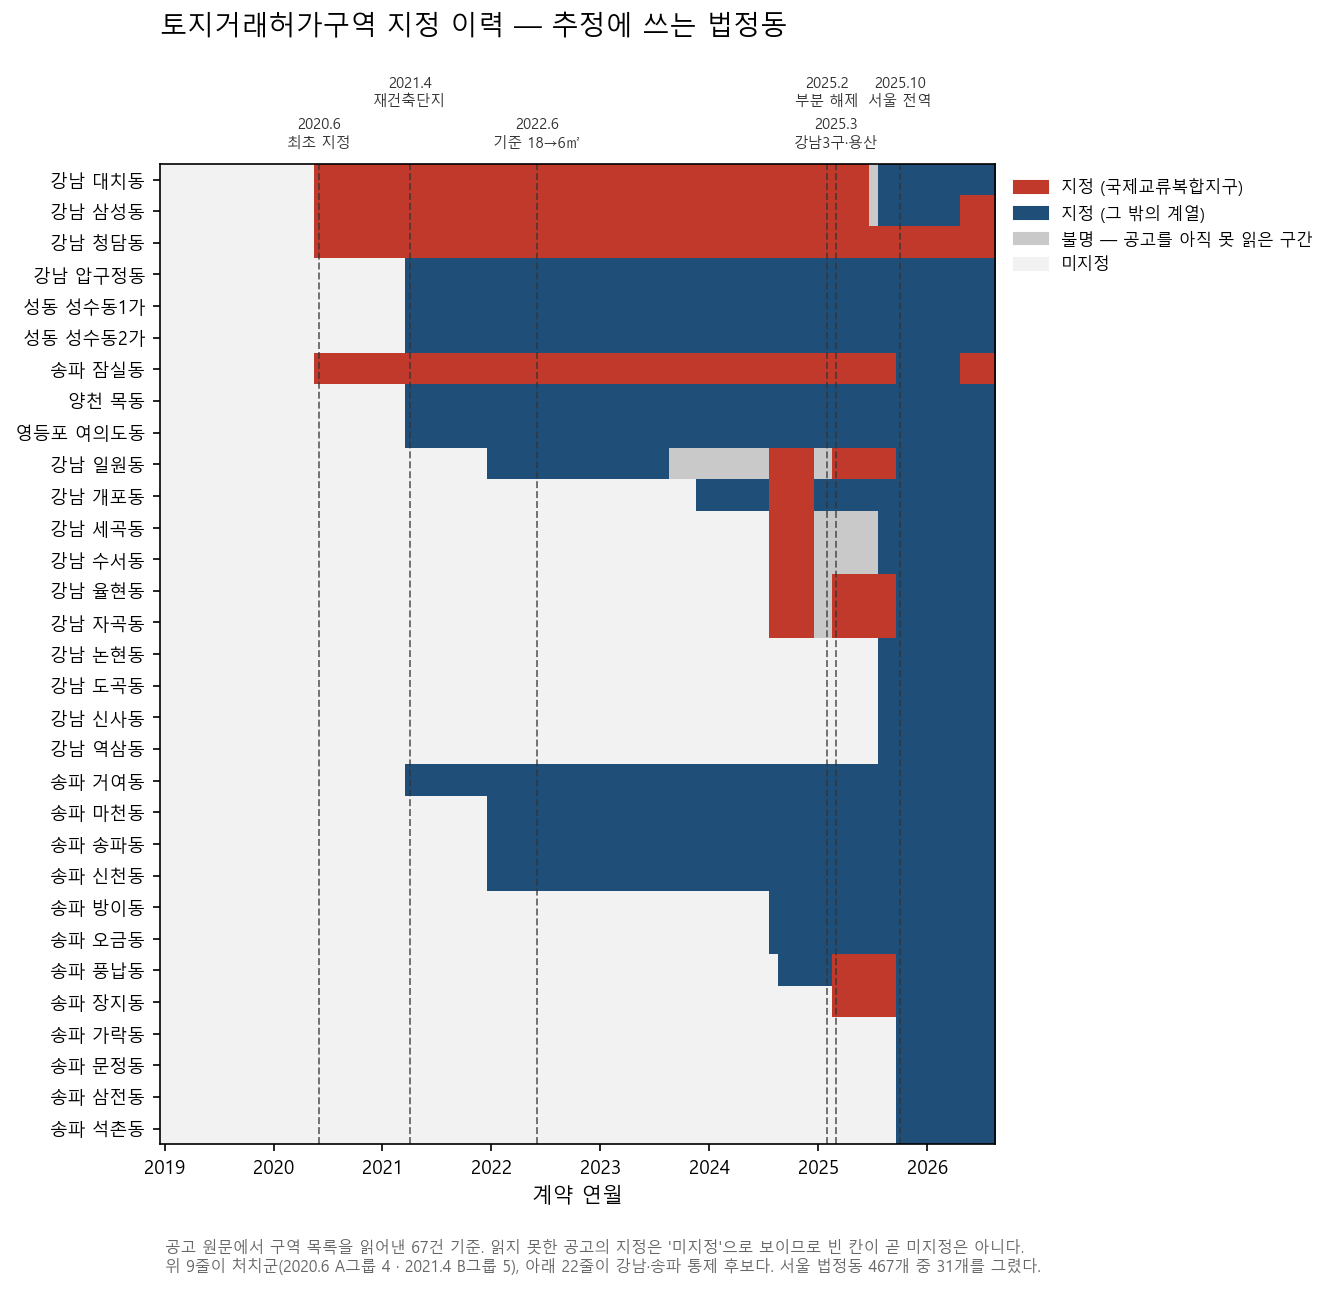
\includegraphics[width=\linewidth]{ltz_heatmap_report.png}
  \caption[토지거래허가구역 지정 이력 --- 추정에 쓰는 법정동]{%
    토지거래허가구역 지정 이력. 가로축은 계약 연월, 한 행이 한 법정동이다.
    \textbf{위 아홉 줄이 처치군}(2020.6 A그룹 넷 · 2021.4 B그룹 다섯),
    아래가 강남·송파 통제 후보다. 붉은색은 국제교류복합지구 계열 지정으로
    A그룹의 처치가 이 계열이다. 점선 여섯이 2.2절의 사건이며,
    \textbf{2025-10 에서 모든 행이 덮이는 것}이 인과 추정을 2025-10-19 에서
    끊는 이유다(0002). 통제 후보 가운데 2025년 이전에 파랗게 칠해지는 동들이
    9.3절에서 빼는 오염 동이다. 회색은 공고 원문에서 구역 목록을 아직 읽어내지
    못한 구간으로, \textbf{빈 칸이 곧 미지정은 아니다}. 서울 전역 467개 동을
    같은 방식으로 그린 것은 \texttt{output/figures/}에 있다.}
  \label{fig:heatmap}
\end{figure}

\subsection{선행연구 세 편과 재현}

2020년 6월 지정을 다룬 국내 연구 세 편을 확인했다. 셋 모두 2025년에 발표됐고,
셋 모두 \textbf{동 단위 집계 자료}를 쓰며, 셋 모두 처치를 \textbf{2020년 6월 단일
사건}으로 취급한다.

말로 비판하는 대신 \textbf{세 편의 사양을 이 연구의 자료로 직접 돌렸다}
(\texttt{scripts/replicate/}). 세 가지가 나왔다.

\textbf{(가) 전상현 외(2025)} --- 동-월 패널 675개(27개 동 $\times$ 25개월)에
구역더미, 시점더미, 교호항, 거래건수를 넣은 OLS다. 같은 격자를 재현하면 거래가
한 건도 없는 \textbf{빈 셀이 31개}이고 전부 통제동이다. 논문 기술통계의 가격
최솟값이 0인 것으로 보아 그 빈 셀을 0으로 코딩한 것으로 보이며, 그렇게 하면 네
계수와 $R^2$가 모두 논문값에 근사하게 재현된다(교호항 $+0.3549$, 논문
$+0.2928$). 그런데 \textbf{빈 셀을 정상적으로 제외하면 교호항이 $-0.0448$로
부호가 뒤집힌다.} 거래가 없는 달의 ``평균 가격''은 0이 아니라 결측이다.

같은 논문이 \textbf{거래건수를 통제변수로} 넣은 것도 문제다. 거래량 감소는
정책의 결과이므로 통제하면 효과의 일부를 빨아들인다. 빼면 교호항이 $-0.1121$
($p=0.002$), 동·월 고정효과까지 넣으면 $-0.1215$가 된다.

\textbf{(나) 이한웅·이춘원(2025)} --- 잠실동을 처치, 송파구 나머지 동을 통제로
두었다. 본문은 이중차분을 표방하나 \textbf{보고된 $t$-검정은 각 집단 내부의
사전-사후 비교}이며 이중차분 계수가 아니다. 논문 표의 수치로 차이의 차이를 직접
계산하면 $\pm$3개월 $+12.2$\,\%p, $\pm$6개월 $-2.9$\,\%p, $\pm$12개월
$-3.9$\,\%p로 \textbf{$\pm$6개월부터 부호가 바뀐다}. 잠실동 가격이 유의하게
올랐다는 것은 맞지만, 통제동도 함께 그리고 더 많이 올랐다.

\textbf{(다) 양지영·정준호(2025)} --- 합성대조군법을 썼다. 도너 풀 15개 동 가운데
\textbf{압구정동·성수동1가·성수동2가가 2021년 4월 27일 토허구역으로 지정}됐다.
연구기간 2018-06$\sim$2022-05 중 마지막 13개월 동안 도너의 20\%가 처치를 받은
상태였다. 처치받은 단위를 도너 풀에 두면 반사실 경로가 왜곡된다
\citep{abadie2010synthetic}.

\subsection{왜 결론이 갈렸는가 --- 설계 선택의 분해}

세 편은 서로 다른 결론을 냈다. 전상현은 가격에 영향이 없다고, 이한웅은 올랐다고,
양지영은 억제됐다고 적었다. \textbf{이것이 실질적 차이인가 설계 선택의
산물인가}가 이 연구의 네 번째 연구 질문이다.

이를 답하려고 \textbf{사양 곡선}\citep{simonsohn2020specification}을 썼다.
합리적인 설계 선택을 전부 조합해 한 그림에 놓는 방법이다. 축은 이 연구가 실제로
내린 결정에서 왔고, 각 축의 대안은 \textbf{선행연구가 실제로 쓴 것이거나 이
연구가 고치기 전에 쓰던 것}이다. 지어낸 대안이 아니다.

\[
\underbrace{2}_{\text{처치군}} \times \underbrace{4}_{\text{통제군}}
\times \underbrace{3}_{\text{창}} \times \underbrace{2}_{\text{사건정렬}}
\times \underbrace{2}_{\text{빈칸}} \times \underbrace{2}_{\text{척도}}
= 192 \;\text{가지}
\]

192가지 전부에서 거래량 효과가 음수였다(9.5절). 여기서 중요한 것은 그 사실이
아니라 \textbf{무엇이 추정치의 크기를 갈랐는가}다. 축마다 그 축의 값들이 내는
중위 추정치의 최대 차이를 재면 표~\ref{tab:rq4-axes}와 같다.

% 자동 생성 — scripts/build_tables.py. 손으로 고치지 않는다.
% 출처: output/results/05b_spec_curve.json : 축별_영향.거래량
\begin{table}[htbp]
  \centering
  \caption{설계 선택이 추정치를 가르는 폭 (거래량, 지정 직후 3개월). 사건 시점 정렬이 통제군 정의의 17배다.}
  \label{tab:rq4-axes}
  \begin{tabular}{lr}
    \toprule
    \textbf{설계 선택} & \textbf{추정치 폭 (\%p)} \\
    \midrule
    사건정렬 & 39.6 \\
    척도 & 11.4 \\
    처치군 & 6.7 \\
    통제군 & 2.3 \\
    창 & 1.1 \\
    빈칸 & 0.9 \\
    \bottomrule
  \end{tabular}

  \begin{minipage}{\linewidth}\footnotesize
  \textit{주.} 축별로 그 축의 값들이 내는 중위 추정치의 최대 차이. 달력 월 $-40.5\%$ 대 효력일 $-80.1\%$.
  \end{minipage}
\end{table}


\textbf{사건 시점 정렬이 통제군 정의의 17배다.} 구체적으로 달력 월로 자르면
중위 $-40.5\%$, 효력일에 맞추면 $-80.1\%$다. 지정 효력일이 6월 23일인데 달력
월로 묶으면 2020년 6월 한 칸에 지정 전(1$\sim$22일)과 후(23$\sim$30일)가 섞인다.
실제로 강남·송파의 해당 칸 3,343건 중 1,532건(45.8\%)이 지정 전 거래였다.

\textbf{선행연구끼리 결론이 엇갈린 이유는 지역을 어떻게 나눴느냐가 아니라
날짜를 어디에 맞췄느냐에서 왔다.} 통제군 정의는 2.3\,\%p밖에 가르지 않는다.
세 편이 서로 다른 지역 정의를 쓴 것은 결론 차이의 원인이 아니다.

\subsection{차별점}

이 연구와 선행연구 세 편의 차이를 정리하면 다음과 같다.

\begin{table}[htbp]
  \centering
  \caption{선행연구 세 편과의 차이}
  \label{tab:diff}
  \begin{tabular}{lllll}
    \toprule
    \textbf{항목} & \textbf{전상현 외} & \textbf{이한웅·이춘원} &
    \textbf{양지영·정준호} & \textbf{본 연구} \\
    \midrule
    분석 단위 & 동-월 집계 & 동 패널 & 동 패널 & \textbf{거래 단위} \\
    물건 특성 통제 & 없음 & 불명 & 세대수·건축연도 &
      \textbf{면적·층 + 단지 FE} \\
    사건 시점 정렬 & 달력 월 & 달력 & 달력 & \textbf{효력일} \\
    처치 구조 & 2020.6 단일 & 2020.6 단일 & 2020.6 단일 &
      \textbf{2020/2021/2025} \\
    2021.4 지정 & --- & --- & \textbf{미반영(도너 오염)} & 반영 \\
    사전추세 검정 & 없음 & 필요성만 언급 & SCM 사전적합 &
      \textbf{사건연구 + 민감도} \\
    거래량 & \textbf{통제변수로 사용} & 기술통계 & --- & \textbf{주 결과변수} \\
    코드 공개 & --- & --- & --- & \textbf{전 과정} \\
    \bottomrule
  \end{tabular}
\end{table}

가장 뚜렷한 두 지점은 \textbf{처치 역전}과 \textbf{동일 동 내 파급효과}다. 처치
역전 자체는 방법론적으로 확립되어 있고\citep{dechaisemartin2020twoway} 적용
사례도 있다. 이 사례의 특징은 역전 간격이 \textbf{39일}로 극히 짧아 거시 환경과
계절성이 사실상 고정되어 있었다는 점, 그리고 해제가 전면적이 아니라 부분적이어서
\textbf{같은 동 안에 규제 상태가 다른 단지가 공존}한다는 점이다. 뒤쪽이 7장의
조건이 된다.
